% arara: xelatex
% arara: sage
% arara: xelatex
% arara: clean: {extensions: ['log','out','snm','listing','nav','sage']}
\documentclass[spanish,9pt]{beamer}
\usepackage{euler}
\usepackage{graphicx,hyperref,url, materialbeamer}
\usepackage{braket}
\usepackage{listings}
\usepackage{sagetex}

\graphicspath{ {../img/} }
\setbeamercovered{transparent}
\lstdefinestyle{customsql}{
  belowcaptionskip=1\baselineskip,
  breaklines=true,
  xleftmargin=\parindent,
  language=SQL,
  showstringspaces=false,
  basicstyle=\footnotesize\ttfamily,
  keywordstyle=\bfseries\color{green!40!black},
  commentstyle=\itshape\color{purple!40!black},
  identifierstyle=\color{blue},
  stringstyle=\color{orange},
}
\lstset{escapechar=@,style=customsql}



\usefonttheme{professionalfonts} % using non standard fonts for beamer
%\usefonttheme{serif}

% The title of the presentation:
%  - first a short version which is visible at the bottom of each slide;
%  - second the full title shown on the title slide;
\title[\LaTeX{} \& Friends]{\LaTeX{} \& friends}

% Optional: a subtitle to be dispalyed on the title slide
\subtitle{SageMath, arara, PSTricks \& knitr\\[\baselineskip]
10 de noviembre del 2018}

% The author(s) of the presentation:
%  - again first a short version to be displayed at the bottom;
%  - next the full list of authors, which may include contact information;
\author[Dimension R]{Carlos Aznarán} 

%\titlegraphic{
\includegraphics[width=\textwidth]{usa}}

\institute[Universidad Nacional de Ingeniería]{
Matemáticas\\
  Facultad de Ciencias\\
  Universidad Nacional de Ingeniería}

\date[\today]{
 \today}

\providecommand{\di}{\mathop{}\!\mathrm{d}}
\providecommand*{\der}[3][]{\frac{d\if?#1?\else^{#1}\fi#2}{d #3\if?#1?\else^{#1}\fi}} 
 \providecommand*{\pder}[3][]{% 
    \frac{\partial\if?#1?\else^{#1}\fi#2}{\partial #3\if?#1?\else^{#1}\fi}% 
  }
\renewcommand{\sin}{\mathrm{sen}}
\begin{document}

\begin{frame}
  \titlepage
\end{frame}

\begin{frame}
  \frametitle{\contentsname}

  \tableofcontents
\end{frame}

\section{Background}
\begin{frame}[fragile]
\frametitle{\insertsection}
\end{frame}

\section[\arara]{\arara}

\subsection{¿Qué es esta herramienta?}

\begin{frame}
\frametitle{\insertsection}
\begin{block}{\insertsubsection}
	\begin{itemize}
		\item Herramienta de automatización \TeX{} basada en reglas y directivas.
		\item Control de los documentos: \arara\ no hará algo a menos que le enseñes la tarea y le digas explícitamente la tarea a ejecutar.
	\end{itemize}
\end{block}
\end{frame}

\subsection{Conceptos claves}

\begin{frame}
\frametitle{\insertsection}
\begin{block}{\insertsubsection}
\begin{itemize}
	\item Reglas: Descripción formal de cómo \arara\ maneja una determinada tarea.
	\item Directivas: Comentario especial que se inserta en el código fuente en el que le indicas cómo \arara\ debería comportarse.
	\item Ejemplos de directivas: \texttt{latex}, \texttt{xelatex}, \texttt{luatex}, \texttt{clean}, \texttt{indent}. \texttt{make}, \texttt{xindy}, \texttt{makeglossaries}, incluso puedes crear tus propias directivas.
\end{itemize}
\end{block}
\end{frame}

\subsection{Algunos métodos}

\begin{frame}
\frametitle{\insertsection}
\begin{block}{\insertsubsection}

\end{block}
\end{frame}

\subsection{Cajas de diálogo}

\begin{frame}
\frametitle{\insertsection}
\begin{block}{\insertsubsection}
Es un elemento de control gráfico, generalmente una pequeña ventana, que comunica información al usuario y le solicita una respuesta.
\end{block}
\end{frame}

\begin{frame}[fragile]
\frametitle{\insertsection}
\begin{codebox}{Terminal}{teal}{\icnote}{white}
$ arara hello.tex 
__ _ _ __ __ _ _ __ __ _ 
/ _` | '__/ _` | '__/ _` |
| (_| | | | (_| | | | (_| |
\__,_|_|  \__,_|_|  \__,_|

Processing 'hello.tex' (size: 86 bytes, last modified: 05/03/2018
07:28:30), please wait.

(PDFLaTeX) PDFLaTeX engine .............................. SUCCESS

Total: 0.73 seconds
\end{codebox}
\end{frame}

\section{Sage}
\subsection{Un programa Sage con variables}

\begin{frame}
\frametitle{\insertsection}
\begin{block}{\insertsubsection}
\begin{itemize}
\item Es un sistema computarizado algebraico.
\item Utiliza el lenguaje de propósito general Python.
\item Creado por el matemático de la Universidad de Washington, William Stein, en el año 2005.
\item Sage reutiliza software libre existentes, algunos de ellos son GAP, PARI-GP, Maxima y Singular.
\item Está escrito completamente en Python.
\end{itemize}
\end{block}
\end{frame}

\begin{frame}[fragile]
\frametitle{\insertsection}
\begin{block}{\insertsubsection}
\begin{sageblock}
f(x) = exp(x) * sin(2*x)
\end{sageblock}
The second derivative of $f$ is

\[
\frac{\mathrm{d}^{2}}{\mathrm{d}x^{2}} \sage{f(x)} =
\sage{diff(f, x, 2)(x)}.
\]

Here's a plot of $f$ from $-1$ to $1$:
\end{block}

\begin{sagesilent}
plt  = plot(f, -1, 1)
plt.save("MyPic.pdf")
\end{sagesilent}

\begin{figure}
\centering
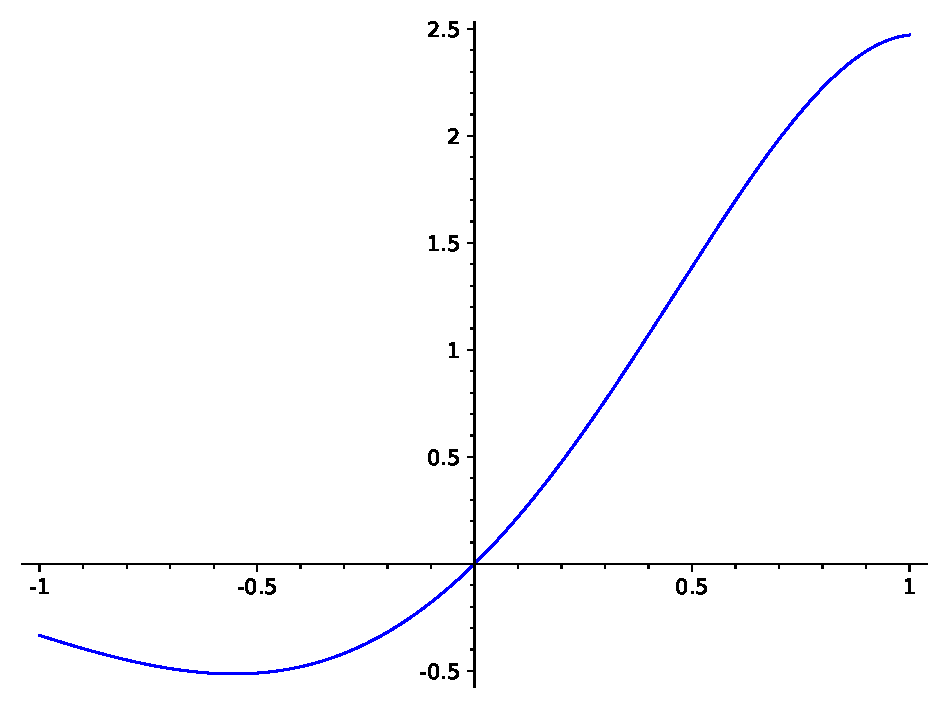
\includegraphics[height=3cm]{MyPic.pdf}
\end{figure}

\end{frame}

\begin{frame}
\begin{block}{Modelo matemático}
Nuestro primer ejemplo se refiere a la programación de un modelo matemático que predice la posición de una pelota lanzada al aire. De la segunda ley de Newton, y asumiendo que la resistencia del aire es insignificante, se puede derivar un modelo matemático que predice la posición $y$ de la pelota en el tiempo $t$.
\end{block}

La declaración $v_0$ = $5$ se llama \emph{asignación}
\end{frame}
%%!TEX root = presentazionelancia.tex
\section{Objetivos}

\begin{frame}
\frametitle{\insertsection}
 	Queremos formar un grupo humano en la UNI alrededor de \LaTeX{} tal como lo hace el Grupo de Usuarios \TeX{} de la Universidad de Tokio.
 	
 	\url{http://ut-tex.org/index.php}
 	\begin{center}
 	
\includegraphics[width=\textwidth]{tokio}		
 	\end{center}
\end{frame}

\begin{frame}[fragile]
\frametitle{¿Cómo lo podemos lograr?}
\onslide<1->
\begin{itemize}
	\item Estudiar los libros de Herbert Voss, vicepresidente del Grupo de Usuarios \TeX{} Germano hablantes.
	\item Conocer herramientas amigas de \LaTeX{} como Sage, arara, PSTricks, knitr y más tecnologías. 
	\item Con el uso de un sistema de control de versiones descentralizado como \texttt{git}
	\item Herramientas de comunicación como \texttt{gitter} o \texttt{Hangouts}.
\end{itemize}
\onslide<2->
Conocimientos previos:
\begin{itemize}
	\item Comandos básicos en \texttt{UNIX}, \LaTeX{} y programación.
\end{itemize}
\end{frame}


%\begin{frame}[fragile]
%\frametitle{Associations}
%    \begin{itemize}
%	\item Typed directed edges between objects (type is denoted by \verb!atype!)
%	\item Identified by source object \verb!id1!, \verb!atype! and destination object \verb!id2!
%	\item Contains data in the form of key-value pairs.
%	\item Contains a 32-bit \verb!time! field.
%	\item Models actions that happen at most once or records state transition (e.g. like)
%	\item Often inverse association is also meaningful (eg like and liked by).
%\end{itemize}
%\end{frame}

%\begin{frame}
%\frametitle{Associations API}
%\begin{itemize}
%\item Add new
%\item Delete
%\item Change type
%\end{itemize}
%Also inverse association is created or modified automatically
%\end{frame}

%\begin{frame}[fragile]
%\frametitle{Querying TAO}
%TAO's associations queries are organized around \emph{associations~ list}
%
%\begin{itemize}
%\item \verb!assoc_get(id1,atype, id2set, high?, low?)!
%\item \verb!assoc_count(id1,atype)!
%\item \verb!assoc_range(id1, atype, pos, limit)!
%\item \verb!assoc_time_range(id1,atype, high, low, limit)!
%\end{itemize}
%
%Query results are bounded to 6000 results
%\end{frame}




%%!TEX root = presentazionelancia.tex
\section{Instalación}
\begin{frame}[t]
\frametitle{\insertsection}
    \onslide<1>\TeX{} Live 2018 \\ \url{https://www.tug.org/texlive/}
    \begin{center}
    	\includegraphics<1>[width=0.8\textwidth]{figs/texlive}
    \end{center}
	\onslide<2>OS GNU/Linux
	\begin{center}
    	\includegraphics<2>[height=0.3\textheight]{figs/tux}
    \end{center}
\end{frame}

%\begin{frame}[fragile]
%\frametitle{Storage Layer}
%\begin{itemize}
%	\item Object and Associations are stored in MySql (before \& with TAO)	
%	\item TAO API is mapped to a small set of SQL queries
%	\item A single MySql server can't handle TAO volumes of data
%	\begin{itemize}
%		\item We divide data into logical \emph{shards}
%		\item \emph{shards} are mapped to db 
%		\item different servers are responsible for multiple shards
%		\item mapping is adjusted for load balancing
%	\end{itemize}
%	\item Object are bounded to a \emph{shard} for their entire lifetime
%	\item Associations are stored in the \emph{shard} of its \verb!id1!
%\end{itemize}
%\end{frame}

%\begin{frame}[c]\frametitle{Cache Layer}
%    TAO cache 
%    \begin{itemize}
%    	\item contains: Objects, Associations, Associations counts
%    	\item implement the complete API for clients
%    	\item handles all the communication with storage layer
%    	\item it's filled on demand end evict the least recently used items
%    	\item Understand the semantic of their contents
%    \end{itemize}
%
%    It consists of multiple servers forming a \emph{tier}
%    \begin{itemize}
%    	\item Request are forwarded to correct server by a \emph{sharding} scheme as dbs
%    	\item For cache miss and write request, the server contacts other caches or db
%    \end{itemize}
%    
%\end{frame}
%\begin{frame}[c]\frametitle{Yet Another caching layer}
%	\onslide<1->\textbf{Problem: }A single caching layer divided into a \emph{tier} is susceptible to \emph{hot spot}
%
%	\onslide<2->\textbf{Solution: }Split the caching layer in two levels
%	\onslide<2->\begin{itemize}
%		\item A \emph{Leader} tier
%		\item Multiple \emph{Followers}	tiers
%	\end{itemize}
%\end{frame}

%\begin{frame}[c]\frametitle{Leaders \& Followers}
%   	\includegraphics[width=\textwidth]{figs/followers_leader.jpeg}
%\end{frame}

%\begin{frame}[c]\frametitle{Leaders \& Followers}
%    \begin{itemize}
%    	\item Followers forward all writes and read cache misses to the leader tier
%		\item Leader sends async cache maintenance messages to follower tier
%		\begin{itemize}
%			\item Eventually Consistent
%		\end{itemize}
%		\item If a follower issues a write, the follower’s cache is updated synchronously
%		\item Each update message has a version number
%		\item Leader serializes writes
%    \end{itemize}
%\end{frame}

%\begin{frame}[c]\frametitle{Leaders \& Followers}
%    \begin{center}
%    \includegraphics<1>[height=0.5\textwidth]{figs/master_slave0.jpg}
%    \includegraphics<2>[height=0.5\textwidth]{figs/master_slave1.jpg}    	
%    \includegraphics<3>[height=0.5\textwidth]{figs/master_slave2.jpg}
%    \end{center}
%    
%\end{frame}

%\begin{frame}[c]\frametitle{Scaling Geographically}
%    \onslide<1->\textbf{Problem: }Network latencies are not low in a multi Data Centers environment
%
%
%    \onslide<2->Considering that read misses are more common than writes in the follower tier
%
%    \onslide<3->\textbf{Solution: }Handles read cache miss locally
%\end{frame}

%\begin{frame}[c]\frametitle{Master \& Slave Regions}
%Fb cluster together DC in regions (with low intra region latency)
%    \begin{itemize}
%    	\item Each region have a full copy of the social graph
%    	\item Region are defined master or slave for each shard
%    	\item Followers send read misses and write requests to the local leader
%    	\item Local leaders service read misses locally
%		\item Slave leaders forward writes to the master shard
%		\item Cache invalidation message are embedded into db replication stream
%        \item Slave leader will update it’s cache as soon as write are forwarded to master
%    \end{itemize}
%\end{frame}

%\begin{frame}[c]\frametitle{Overall Architecture}
%    \begin{center}
%    	\includegraphics[width=\textwidth]{figs/tao_geo_upscaled.png}
%    \end{center}
%
%
%\end{frame}


%%!TEX root = presentazionelancia.tex
\section{Implementation}
%\begin{frame}
%\frametitle{Implementation}
%To achieve performance and storage efficiency Fb have implemented some optimizations to servers.  
%\end{frame}

%\begin{frame}[c]\frametitle{Caching Servers}
%\begin{itemize}
%	\item Memory is partitioned into arenas by association type
%	\begin{itemize}
%		\item This mitigates the issues of poorly behaved association types
%		\item They can also change the lifetime for important associations
%	\end{itemize}
%	\item Small items with fixed size have a lot of pointer overhead
%	\begin{itemize}
%		\item stored separately
%		\item Used for association counts
%	\end{itemize}
%\end{itemize}    
%\end{frame}

%\begin{frame}[fragile]\frametitle{MySql Mapping}
%    We divided the space of objects and associations into \emph{shards}. Each \emph{shard}:
%    \begin{itemize}
%    	\item is assigned to a logical DB
%    	\item there is a table for objects and a table for associations
%    	\item all field of object are serialized in a single \verb!data! column
%    	\item object of different size can be stored in the same column
%    \end{itemize}
%Exceptions:
%\begin{itemize}
%	\item Some object can benefit from being stored in a different table
%	\item Associations counts are stored in a separate table
%\end{itemize}
%\end{frame}

%\begin{frame}[c]\frametitle{Cache Sharding}
%    Shards are mapped to chache server using consistent hashing (like dynamo)
%
%    This can lead to \emph{imbalances}, so TAO use shard cloning to rebalance the load
%
%    There are also \emph{popular object} that can be queried a lot more often than others.
%
%    TAO says to the clients to cache them these objects
%\end{frame}

%\begin{frame}[fragile]\frametitle{High-Degree Objects}
%    Some object have a lot of associations (remember there were a limit of 6000?)
%    \begin{itemize}
%    	\item TAO can't cache all associations list
%    	\item Requests will always end to Db
%    \end{itemize}
%    so
%    \begin{itemize}
%    	\item For \verb!assoc_count!, the edge direction is chosen using the lower degree between source and destination object
%    	\item For \verb!assoc_get! query, only associations whose time~ >~ object's ~creation~ time
%    \end{itemize}
%
%
%
%
%\end{frame}
%%!TEX root = presentazionelancia.tex
\section{Consistency \& Failures}
%\begin{frame}[t]\frametitle{Consistency}
%	Under normal operation, TAO is \emph{eventually consistent}
%
%	Replication lag usually < 1"
%
%	Race conditions are resolved by using version numbers
%
%	In special ``\emph{critical}" situation a read can be forwarded to database to ensure to read from a consistent source of truth. (Useful for auth procedures)
%
%\end{frame}

%\begin{frame}[t]\frametitle{Detecting Failures}
%    Each TAO server stores per-destination time-outs
%    \begin{itemize}
%    	\item if several time-outs occur, hosts are marked as down
%    	\item subsequent requests are aborted
%    	\item Tao reacts trying to route around failures (favouring availability over consistency)
%    	\item Down hosts are actively probed to check if recover
%    \end{itemize}
%    \centering
%    \includegraphics[width=0.6\textwidth]{figs/fail.jpg}
%
%\end{frame}

%\begin{frame}[c]\frametitle{Handling Failures}
%    \begin{description}
%    	\item[Database Fail] Db can crash or be off-line for maintenance. 
%    	\begin{itemize}
%    		\item If master db is down, a slave is promoted to new master
%    		\item If a slave db is down, cache miss are redirected to TAO leaders in master region
%    	\end{itemize}
%    	\item[Leader Fail] Followers re-route requests around it
%    	\begin{itemize}
%    		\item Read miss goes directly to db
%    		\item Write are routed to a random member of the leader tier
%    	\end{itemize}
%    \end{description}
%\end{frame}

%\begin{frame}[c]\frametitle{Handling Failures (2)}
%    \begin{description}
%    	\item[Invalidation Fail] Leader can't contact a follower during a cache invalidation message
%    	\begin{itemize}
%    		\item Leader queues message 
%    		\item If Leader also crash message are lost so new leader send bulk invalidation
%    	\end{itemize}
%    	\item[Follower Fail] Followers in others tiers share the responsibility of it's shard
%    	\begin{itemize}
%    		\item Tao client have a primary tier and a backup tier
%    	\end{itemize}
%    \end{description}
%
%
%\end{frame}

%%!TEX root = presentazionelancia.tex
%\section{Workload \& Performance}
%\begin{frame}[c]\frametitle{Workload}
%\centering
%\includegraphics[width=\textwidth]{figs/table3.pdf}
%
%Frequencies for client request
%
%
%
%\end{frame}

%\begin{frame}[c]\frametitle{Disponibilidad}
%Bajo carga de trabajo real, durante un período de 90 días, la \textbf{fracción de consultas TAO fallidas} es:
%\begin{center}
%	\huge $4.9 \times 10^{-6}$
%\end{center}
%
%\end{frame}
%\begin{frame}[c]\frametitle{Followers Capacity}
%	\centering
%    \includegraphics[width=\textwidth]{figs/followercapacity.pdf}
%\end{frame}

%\begin{frame}[c]\frametitle{Hit Rates and read latency}
%\centering
%\includegraphics[width=\textwidth]{figs/table8.pdf} 
%
%\end{frame}

%\begin{frame}[c]\frametitle{Write Latency}
%   	\includegraphics[width=\textwidth]{figs/writes.pdf}
%\end{frame}

\section{Resumiendo}
\begin{frame}[c]\frametitle{\insertsection}
\begin{description}
	\item[Instalación] \hfill\\
	\begin{itemize}
		\item \TeX{} Live 2018
		\item OS GNU/Linux
		\item Sage 8.4
	\end{itemize}
	\item[Estudio]\hfill\\
	\begin{itemize}
		\item Teoría de los libros
		\item Práctica con ejercicios de ejemplos
	\end{itemize}
	\item[Comunicación y documentación]\hfill\\
	\begin{itemize}
		\item A través de Gitter o Hangout + GitHub.
	\end{itemize}
\end{description}


\end{frame}

\setbeamercolor{background canvas}{bg=matbluedark}
\setbeamercolor{normal text}{fg=white}
\begin{frame}[plain, b]
\centering
\huge \textcolor{white}{¡Gracias por venir!}
\normalsize
\begin{center}
	\includegraphics[width=0.5\textwidth]{Dimensión_R_Logo}\\
\end{center}
\vspace*{\fill}

 \begin{beamercolorbox}[wd=\paperwidth]{section in head/foot}
 \centering\large
\LaTeX{} \& friends -- con el soporte de Dimension R
\vskip10pt
\end{beamercolorbox}
 \end{frame}

\end{document}
